\chapter{Validation}

\section{Introduction}
After building our model inside the \textbf{OMNeT++} we can proceed with the simulation in order to analyze the quantities wich we are interested. First of all we will simulate the model in very simple cases in order to be sure it reproduces the system's behavior correctly. We decided to validate our model by \textit{removing randomness}. This choice allows us to do some easy computation by hand and to verify if the result of simulation is consistent with them. Our model will be considered a good replica of the system if it will pass all the \textit{validation tests}.

\section{1\textsuperscript{st} test: fixed CQI, fixed \(\lambda\) rate, fixed packet size, 1 user}
In this test we just one \texttt{Mobile Station} connected to the antenna wich always generates the same CQI for each timeslot. Inside the \texttt{Web Server} the \(\lambda\) rate is fixed and also the packet size. This is a very simple system with deterministic arrivals and deterministic service demand. We can compute the traffic that \texttt{Web Server} sends to the antenna as \[ th\textsubscript{in} = \frac{packetsize \times 8}{1/(1000\lambda)} \lbrack bps \rbrack \] 
If the system is in a stable state the output throughput and the input throughput must be equal. The maximum output throughput is the one we have by setting all parameters to maximum values. \[ th\textsubscript{max} = \frac{\#RB \times RBsize\textsubscript{max} \times 8}{T\textsubscript{slot}} = \frac{25 \times 93 \times 8}{0.001} = 18.6 \textnormal{ Mbps} \] We can derive very easily the \(\lambda\textsubscript{max}\) rate wich produces the max throughput allowed by antenna. \[\lambda\textsubscript{max} = \frac{\#RB \times RBsize\textsubscript{max}}{1000 \times T\textsubscript{slot} \times packetsize\textsubscript{max}} = \frac{25 \times 93}{1000 \times 0.001 \times 75} = 31 \textnormal{ ms\textsuperscript{-1}} \] For \( 0<\lambda<\lambda\textsubscript{max} \) the system is a stable state and so \(th\textsubscript{in} = th\textsubscript{out}\). For higher \(\lambda\) the FIFOQueue grows indefinitely because the frame is not able to carry as much data in a time slot.

Let's consider all the simulations with the following parameters:
\begin{itemize}
	\item \(\lambda \in \{1,2,\ldots,32\}\)
	\item \(packetsize=75\)
	\item \(CQI=15\)
\end{itemize}
  We can se in the graph a linear behavior regarding the throughput until the system is not saturated. Note that the response time for each packet is zero since there is no queueing until \(\lambda < \lambda\textsubscript{max}\) and grows indefinitely when the system saturates. This is not surprising since \(th\textsubscript{in} \propto \lambda\) when \(\lambda < \lambda\textsubscript{max}\) and packet's size is fixed.
\begin{figure}[H]
  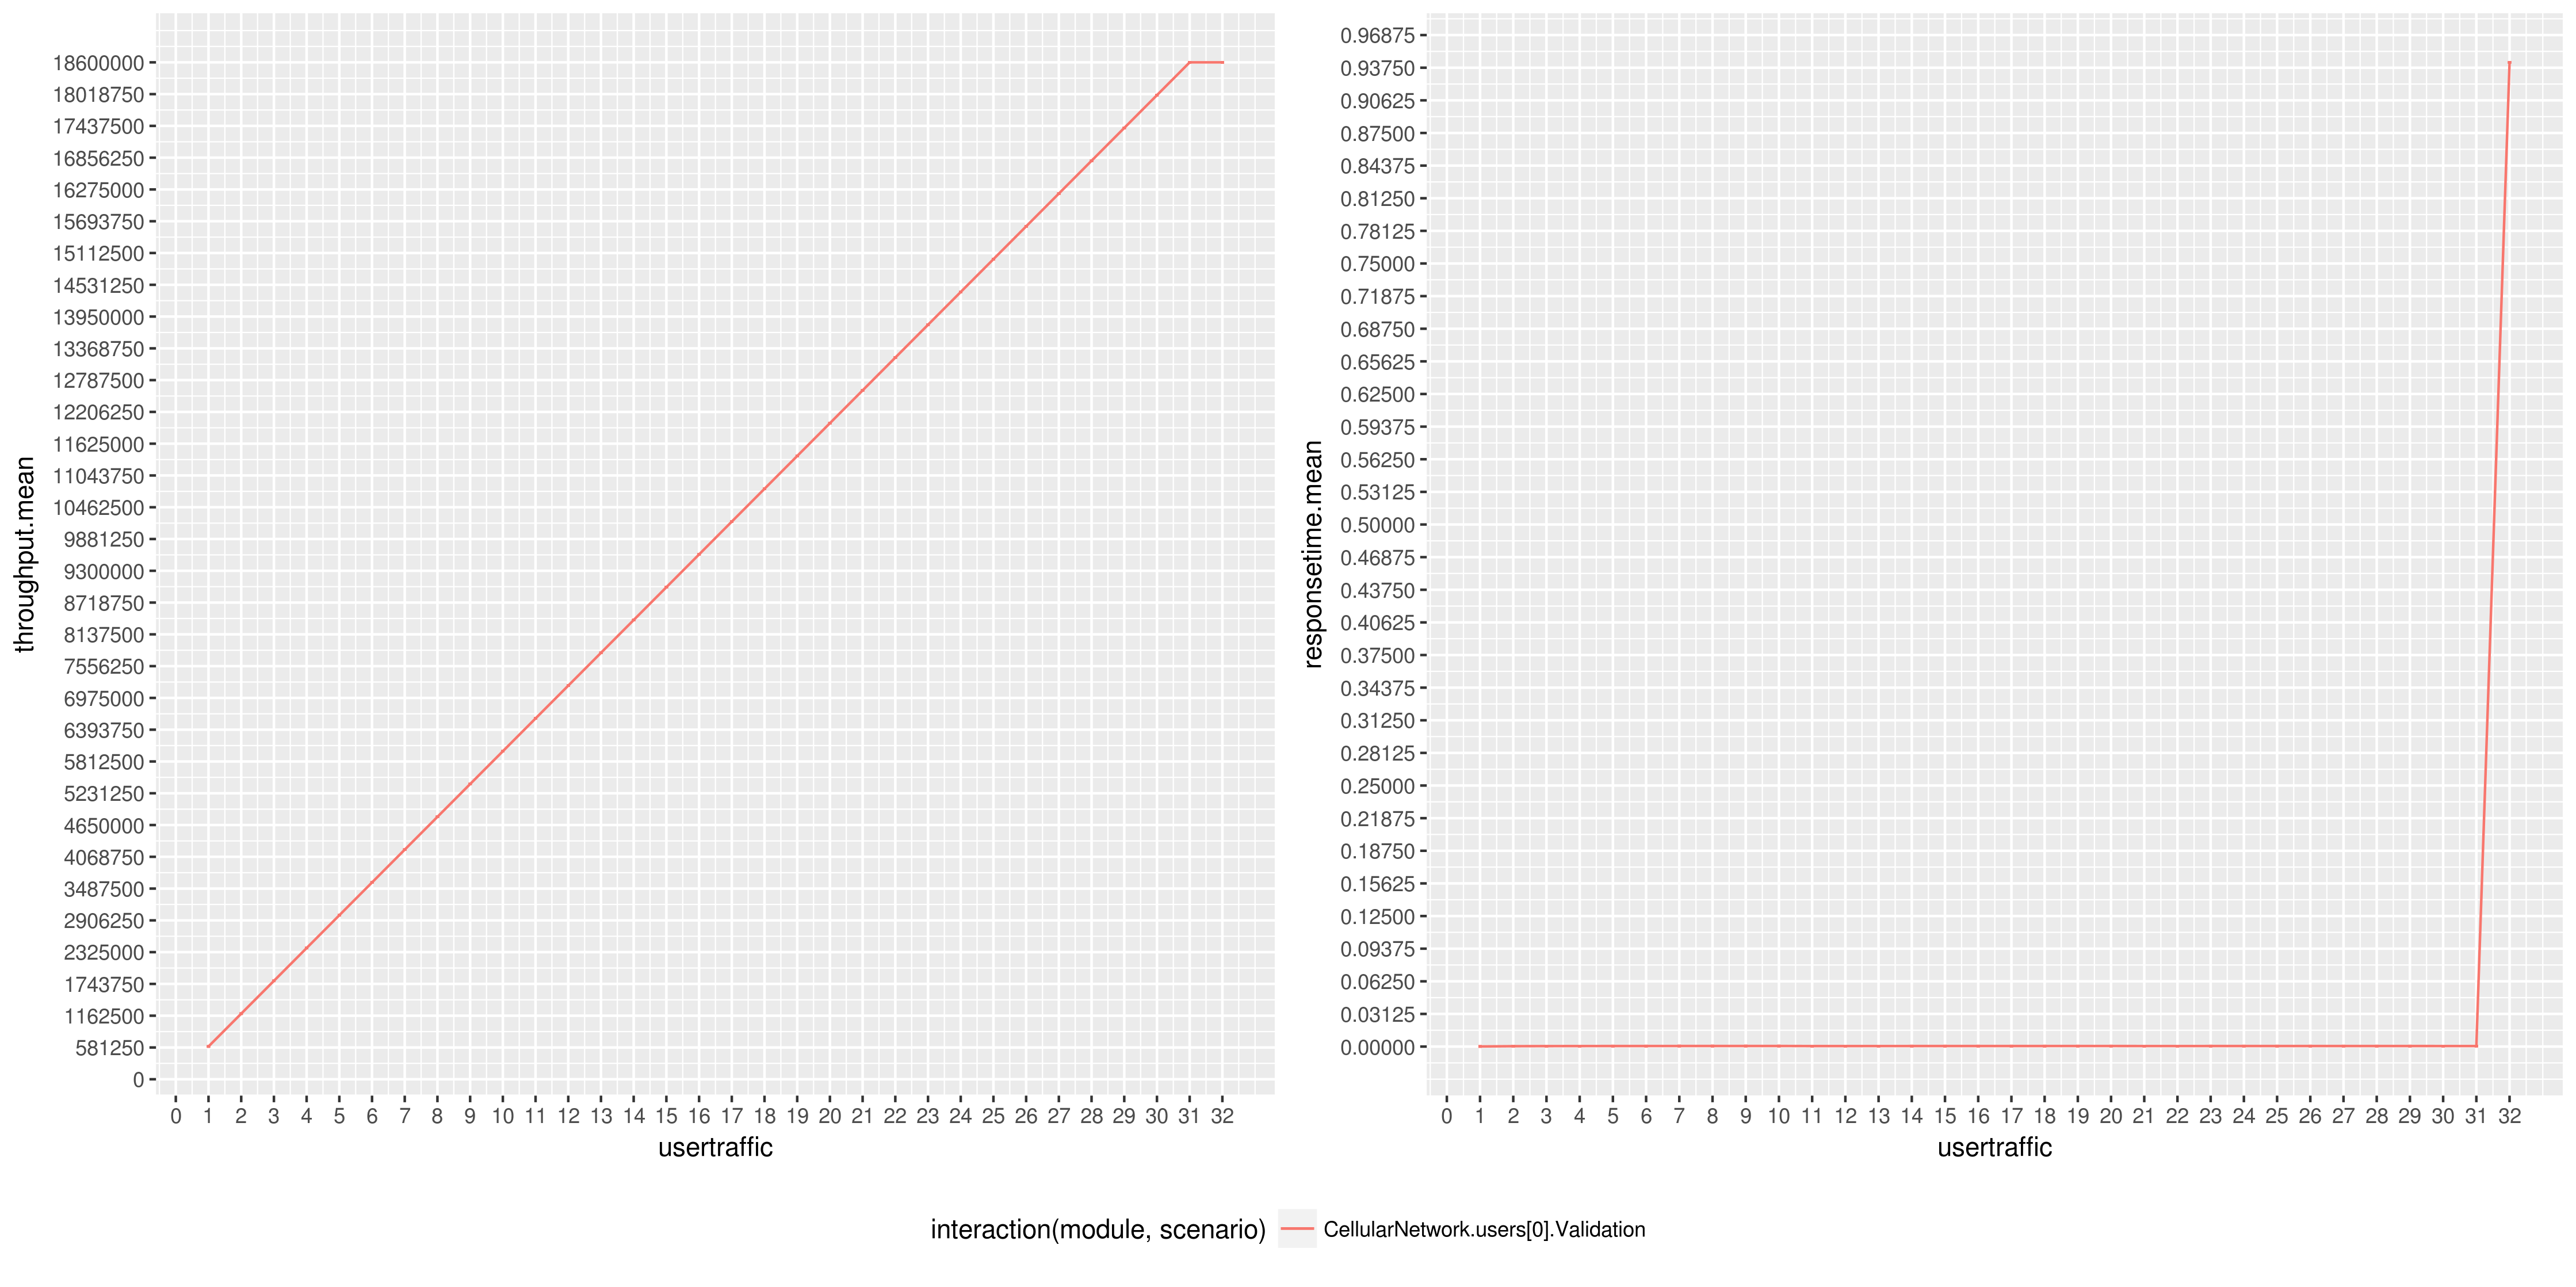
\includegraphics[width=1\textwidth]{images/plotvalidation}
  \caption{throughput, validation scenario}
  \label{fig:throughput, validation scenario}
\end{figure}

\section{2\textsuperscript{nd} test: fixed CQI, fixed \(\lambda\) rate, fixed packet size, 2 users}
In this test there are two \texttt{Mobile Stations} connected to antenna. As in the previous scenario all parameters are fixed. We have two indipendent flow of data from \texttt{Web Servers} to \texttt{Antenna} so the input throughtput could by computed as
\[ th\textsubscript{in} = \frac{packetsize\textsubscript{0} \times 8}{1/(1000\lambda\textsubscript{0})} + \frac{packetsize\textsubscript{1} \times 8}{1/(1000\lambda\textsubscript{1})}\]
For these simulation we have chosen the following parameters:
\begin{itemize}
	\item \(packetsize\textsubscript{0} = packetsize\textsubscript{1} = 32\)
	\item \(CQI\textsubscript{0} = 6\)
	\item \(CQI\textsubscript{1} = 15\)
	\item \(\lambda = \lambda\textsubscript{0} = \lambda\textsubscript{1}\) and \(\lambda \in \{1,2,\ldots,32\}\)
\end{itemize}
In thise case we will simulate and then we will analyze the results.